\documentclass{report}
% Comment the following line to NOT allow the usage of umlauts
\usepackage[utf8]{inputenc}
\usepackage[francais]{babel}
\usepackage{listings}
\usepackage{xcolor}
\usepackage{textcomp}
\usepackage{graphicx}
\pagestyle{plain}
\definecolor{listinggray}{gray}{0.9}
\definecolor{lbcolor}{rgb}{0.9,0.9,0.9}
\lstset{
 backgroundcolor=\color{lbcolor},
 tabsize=4,
 rulecolor=,
 language=matlab,
 basicstyle=\scriptsize,
 upquote=true,
 aboveskip={1.5\baselineskip},
 columns=fixed,
 showstringspaces=false,
 extendedchars=true,
 breaklines=true,
 prebreak = \raisebox{0ex}[0ex][0ex]{\ensuremath{\hookleftarrow}},
 frame=single,
 showtabs=false,
 showspaces=false,
 showstringspaces=false,
 identifierstyle=\ttfamily,
 keywordstyle=\color[rgb]{0,0,1},
 commentstyle=\color[rgb]{0.133,0.545,0.133},
 stringstyle=\color[rgb]{0.627,0.126,0.941},
}
% Start the document
\begin{document}
\newpage

%%%
% PARTIE Interface Graphique
%%%
\chapter{Partie Interface Graphique}
\section{Présentation}
La partie Interface Graphique comprend principalement l'habillage visuel des éléments avec lequel l'utilisateur va interagir pour jouer au jeu. MetaBot étant un jeu pour "programmeur", le joueur interagi surtout avec le menu principal et l'éditeur de comportement afin de créer des équipes pour pouvoir les faire s'affronter.
\paragraph{}
L'interface graphique que nous avons créé se décompose en quatre parties, le menu principal, le menu de paramètre, l'éditeur de comportement et des fonctionnalités directement en jeu.
\paragraph{}
Le premier choix a donc été de revoir totalement l'interface, ce que nous pouvions faire grâce aux nouveaux éléments apportés. En effet il fallait rajouter de nouvelles fonctionnalités basiques à cette interface qui en avait finalement très peu et ajouter un peu de couleurs à tout ça.


\section{Menu Principal}
\paragraph{}
Voici l’écran de menu principal. Ceci est le premier écran qui apparaîtra lorsque vous lancerez le jeu.
Passons en revue toutes les possibilités que ce menu offre.
\subsection{Lancer une Partie}
En cliquant sur ce bouton, la partie se lancera, et le combat pourra commencer !

\begin{figure}[!h]
	\centering
		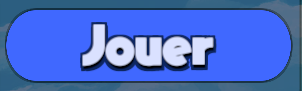
\includegraphics[scale=0.65]{BoutonJouer}
	\caption{Bouton Jouer}
\end{figure}
\subsection{Bouton Editeur de Comportement}
Ce bouton vous mènera à l’éditeur de comportement, pour gérer le comportement des unités de vos équipes.

\begin{figure}[!h]
	\centering
		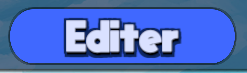
\includegraphics[scale=0.80]{Bouton_Editer}
	\caption{Bouton Éditer}
\end{figure}
\subsection{Bouton Paramètre}
Voici le menu paramètres, qui offre plusieurs choix de personnalisations.

\begin{figure}[!h]
	\centering
		
\includegraphics[scale=0.80]{Bouton_Parametre}
	\caption{Bouton Paramètre}
\end{figure}
\subsection{Choisir le nombre d'équipe}
Permet de choisir le nombre de joueurs. 2 joueurs minimum, 4 maximum.

\begin{figure}[!h]
	\centering
		
\includegraphics[scale=0.60]{Selection_nb_joueurs}
	\caption{Sélection du nombre de joueur}
\end{figure}
\subsection{Choisir les équipes}
Choix des équipes pour chaque joueur.

\begin{figure}[!h]
	\centering
		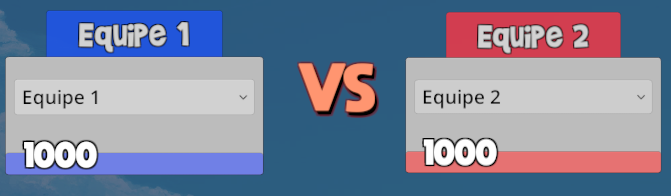
\includegraphics[scale=0.60]{Selection_Equipes}
	\caption{Sélection de l'équipe}
\end{figure}
\subsection{Bouton "Reload Team"}
Ce bouton permet de recharger les équipes.
\subsection{Bouton pour quitter le jeu}
Ce bouton ouvre une boite de dialogue demandant à l'utilisateur si il veut vraiment quitter le jeu. Il peut ainsi choisir de revenir sur le menu principal ou de fermer le jeu.
\subsection{Choisir carte de jeu}
Vous permet de choisir entre plusieurs cartes de jeu.

\begin{figure}[!h]
	\centering
		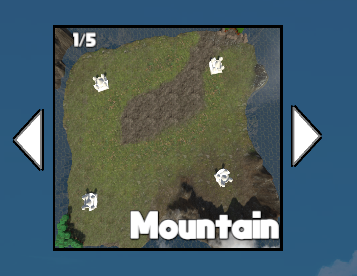
\includegraphics[scale=0.80]{Selection_Map}
	\caption{Sélection de la carte de jeu}
\end{figure}
\subsection{Choisir nombre de départ de chaque unités}
Détermine, pour chaque unité, le nombre avec lequel vous commencerez la partie.

\begin{figure}[!h]
	\centering
		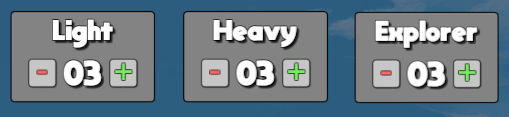
\includegraphics[scale=0.80]{Nombre_Unit}
	\caption{Choix du nombre d'unités}
\end{figure}


\subsection{Paramètres}
Voici le menu paramètres, qui offre plusieurs choix de personnalisations.
\begin{figure}[!h]
	\centering
		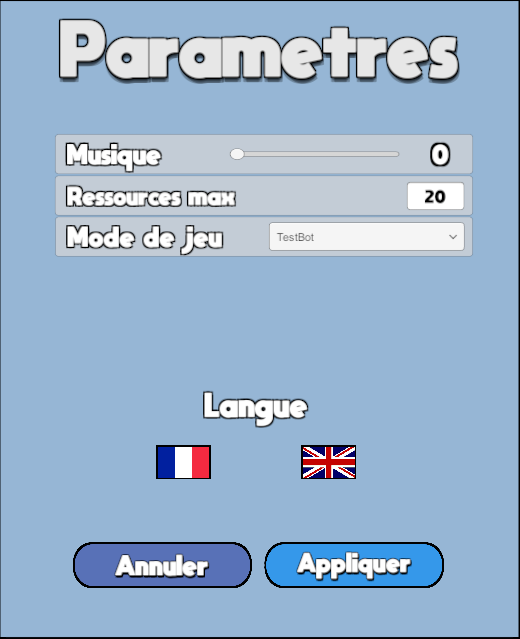
\includegraphics[scale=0.50]{Ecran_Parametre}
	\caption{Écran Paramètres}
\end{figure}


\subsection{Changer le Volume de la musique}
Permet de régler le volume du jeu
\begin{figure}[!h]
	\centering
		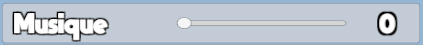
\includegraphics[scale=0.80]{Control_Musique}
	\caption{Volume de la musique}
\end{figure}


\subsection{Choisir nombre de ressource maximum dans le jeu}
Cette option vous permet de définir le nombre maximal de ressources présentes au même moment sur le sol
\begin{figure}[!h]
	\centering
		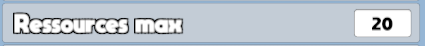
\includegraphics[scale=0.80]{Limite_Ressources}
	\caption{Nombre de ressource maximum}
\end{figure}


\subsection{Choisir le mode de jeu}
Vous pouvez sélectionner le mode de jeu que vous désirez.
\subsubsection{TestBot}
Le mode par défaut.
\begin{figure}[!h]
	\centering
		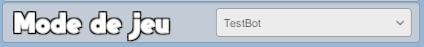
\includegraphics[scale=0.80]{ModeJeuTestBot}
	\caption{Choix du mode de jeu}
\end{figure}


\subsubsection{RessourceRace}
Deux nouvelles options apparaissent sous ce mode :
\begin{figure}[!h]
	\centering
		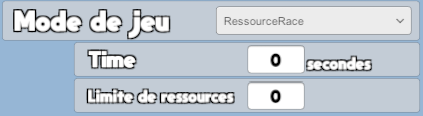
\includegraphics[scale=0.80]{ModeJeuRessourceRace}
	\caption{Options du mode RessourceRace}
\end{figure}

Temps: \newline
Vous permet de choisir la durée maximale d’une partie/\newline

Limite de ressources:\newline
La condition de victoire. La première équipe à avoir atteint cette limite remporte la partie

\subsection{Choisir la langue}
Choisissez la langue que vous préférez, simplement en cliquant sur le drapeau correspondant.
\begin{figure}[!h]
	\centering
		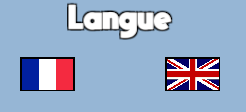
\includegraphics[scale=0.80]{Choix_Langue}
	\caption{Choix de la langue}
\end{figure}


\subsection{Bouton Retour}
Ce bouton annule tous les changements qui ont pu être fait, et vous renvoie au menu principal
\subsection{Bouton Valider}
Ce bouton valide les paramètres, puis vous renvoie au menu principal.
\begin{figure}[!h]
	\centering
		
\includegraphics[scale=0.80]{ApplyCancelSettings}
	\caption{Annuler ou Appliquer les changements}
\end{figure}
\clearpage






\section{Editeur de Comportement}
Cet écran vous permet d’éditer le comportement des unités de vos équipes.
\begin{figure}[!h]
	\centering
		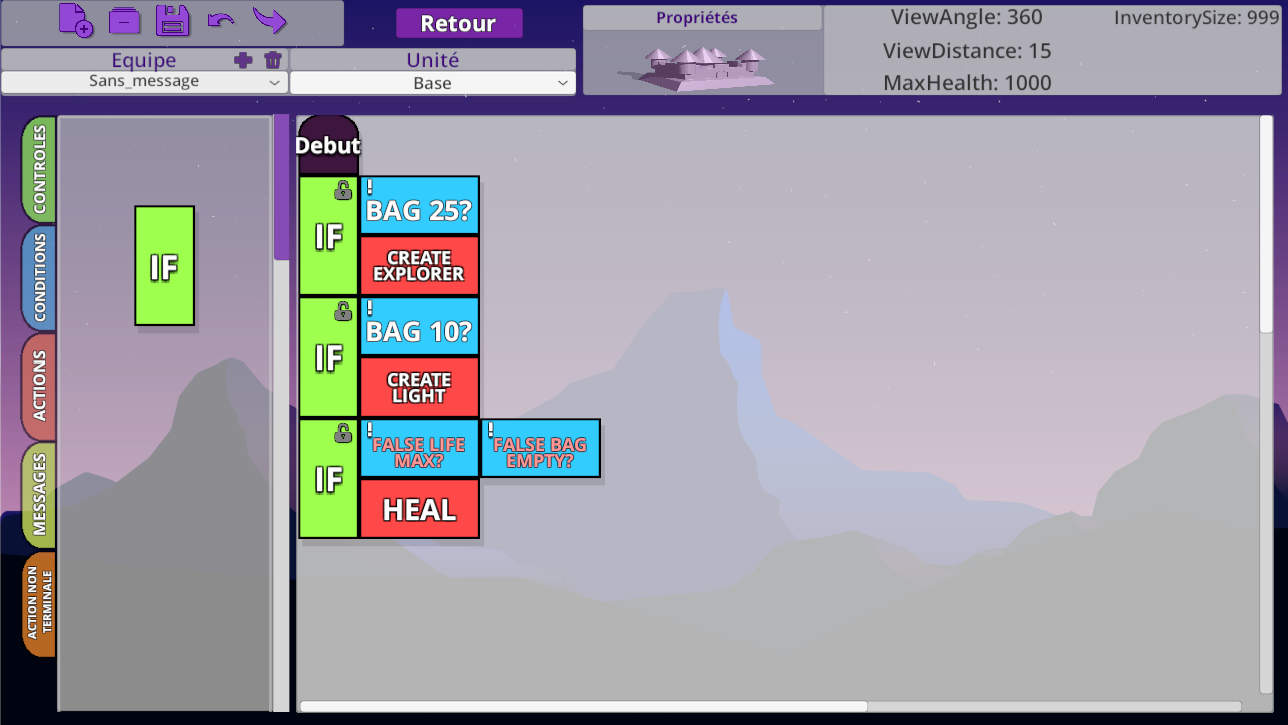
\includegraphics[scale=0.35]{Ecran_Editeur}
	\caption{Écran de l'éditeur}
\end{figure}
% ToolBox %

\subsection{Bouton Nouveau Comportement}
Ce bouton vous permet d’ouvrir un nouveau comportement vide, écrasant le comportement actuellement traité
\subsection{Bouton Chargement Comportement}
Permet de charger le comportement de l’unité active
\subsection{Bouton Sauvegarde du Comportement}
Permet de sauvegarder le comportement de l’unité en cours d’édition
\subsection{Bouton "Undo"}
Permet d’annuler la dernière création ou suppression de pièce
\subsection{Bouton "Redo"}
Permet de restituer la dernière annulation
\subsection{Bouton de retour au menu principal}
Renvoie au menu principal
% IMAGE TOOLBOX
\begin{figure}[!h]
	\centering
		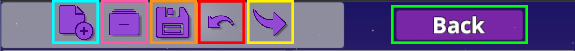
\includegraphics[scale=0.80]{ToolBoxSelectedArea}
	\caption{Boutons de la ToolBox}
\end{figure}

% Equipe + Unité %
\subsection{Choix de l'équipe}
Ce menu déroulant vous permet de choisir l’équipe sur laquelle travailler.
\subsection{Choix de l'unité}
Permet de créer une nouvelle équipe.
% IMAGE TEAM + UNIT
\begin{figure}[!h]
	\centering
		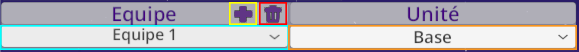
\includegraphics[scale=0.80]{Team_UnitSelectedArea}
	\caption{Sélection équipe et unité}
\end{figure}


\subsection{Bouton Création d'équipe}
Permet de créer une nouvelle équipe.
\subsection{Bouton Suppression d'équipe}
Permet de supprimer l’équipe actuellement sélectionnée.
\subsection{Affichage du modèle 3D de l'unité courante}
La zone en violet représente le modèle de l'unité actuellement sélectionnée.
\subsection{Affichage des statistiques de l'unité courante}
La zone en bleu affiche ses statistiques.
%IMAGE STATS + MODEL
\begin{figure}[!h]
	\centering
		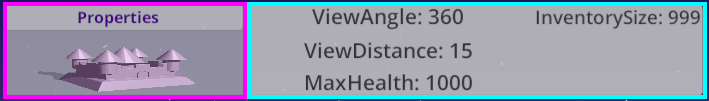
\includegraphics[scale=0.60]{StatsModeleUnitSelectedAreas}
	\caption{Statistiques et modèle de l'unité}
\end{figure}


% Zone de création des comportements
\subsection{Pièces de comportement}


\begin{minipage}{0.4\linewidth}
\paragraph{}
Ici se trouve la totalité des pièces à votre disposition pour la création de comportements.
Les pièces sont classées par type.
\end{minipage}
\begin{minipage}{0.2\linewidth}
\
\end{minipage}
\begin{minipage}{0.4\linewidth}
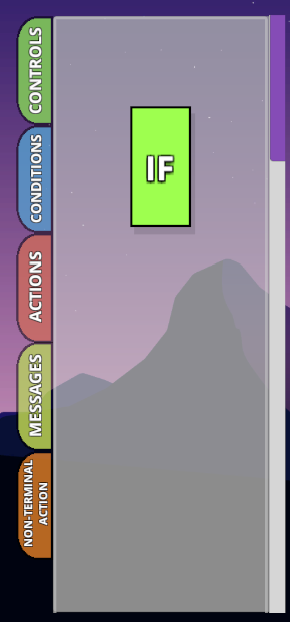
\includegraphics[scale=0.40]{Pieces}
\end{minipage}\hfill





\subsection{Zone d'édition}
Zone de création et d’édition de comportement.
\begin{figure}[!h]
	\centering
		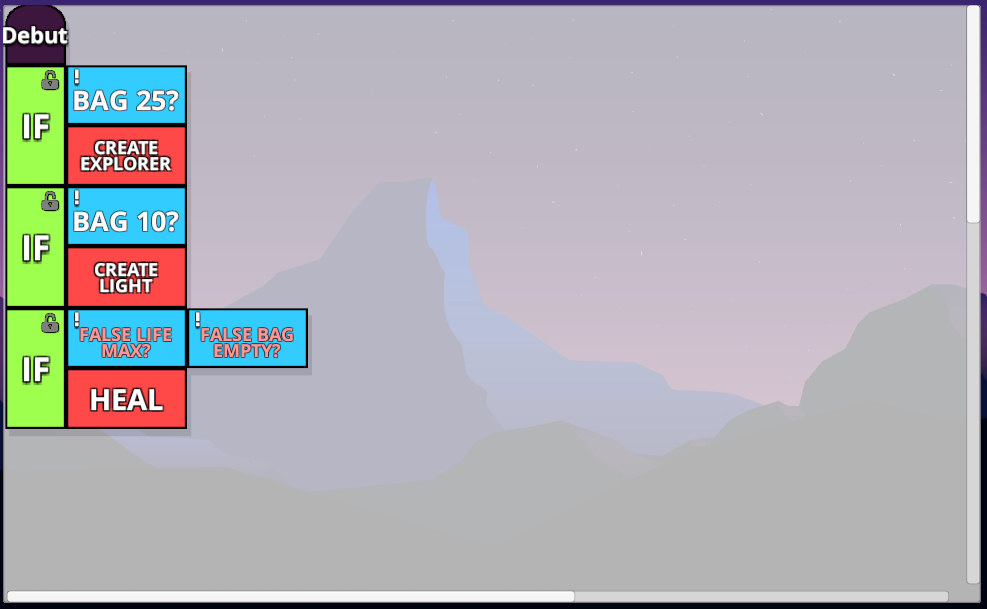
\includegraphics[scale=0.40]{Editeur}
	\caption{Éditeur de comportement}
\end{figure}


\section{Element dans le jeu}
\subsection{Réglage du volume du son}
Permet de régler le son durant une partie.
\begin{figure}[!h]
	\centering
		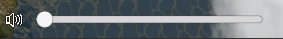
\includegraphics[scale=0.80]{SoundIG}
	\caption{Volume du son en jeu}
\end{figure}
\end{document}
